% !TEX root=../main.tex
\documentclass[beamer]{standalone}
\begin{document}
% ==============================================================
% Method
% ==============================================================
\newminted{python}{fontsize=\scriptsize, 
		   linenos,
		   numbersep=8pt,
		   gobble=1,
		   frame=lines,
		   bgcolor=bg,
		   framesep=3mm} 

\defverbatim[colored]\exampleCode{
\begin{pythoncode}
   with torch.no_grad():
       # only the parameter vertex available
       l = igl.cotmatrix(v, f)
       m = igl.massmatrix(v, f, igl.MASSMATRIX_TYPE_BARYCENTRIC)
       # to pytorch
       l = torch.from_numpy(l.toarray()) 
       m = torch.from_numpy(m.toarray())

       # this is the same fomulation as laplacian smoothing
       i_L = (torch.eye(l.shape[1]) + 10*step_size * (m-10*l)).to(device='cuda')
       g = i_L.inverse() @ grad
   ...
   # reparameterization: x(u) = (I + \lambda L)_inv u
   param = l_p.inverse() @ param
\end{pythoncode}
}

\begin{frame}{Method}
\framesubtitle{Implementation of the previous work: Mesh case}
    \begin{itemize}
        \item iterative form
        \begin{equation}
                x \leftarrow x - \eta \textcolor{red}{(I + \lambda L)^{-p}} {\diffp{\Phi}{x}}
        \end{equation}
        \item Code
        \begin{itemize}
            \item Solve laplacian smoothing every iteration
        \end{itemize}
    \end{itemize}

    \exampleCode

% note %
\note[item]{
}
\end{frame}

\begin{frame}{Method}
    \framesubtitle{Implementation of the previous work: Mesh case}

        \begin{figure}
            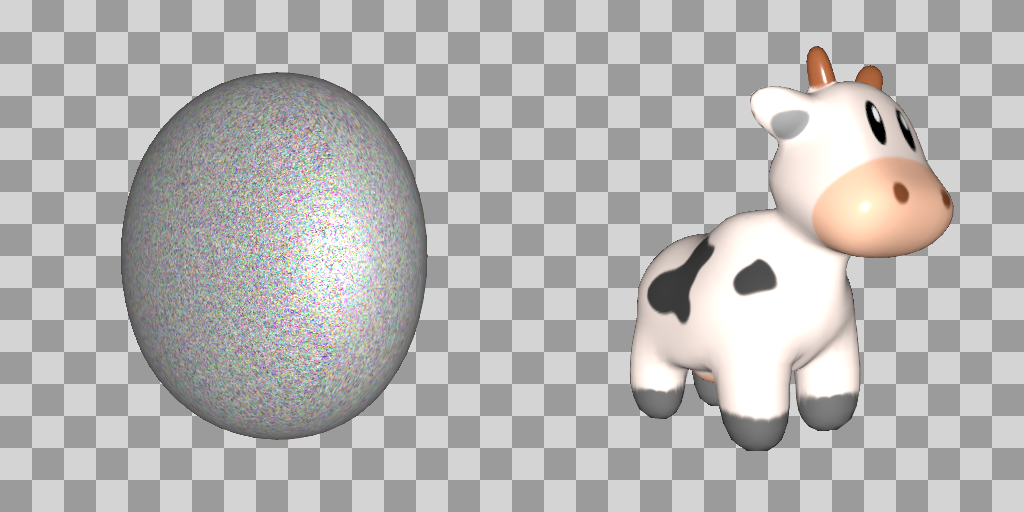
\includegraphics[width=0.25\linewidth]{./figures/spot.png}
        \end{figure}

        \begin{figure}
            \centering
            \begin{columns}[t]
                \column[]{.25\textwidth}
                    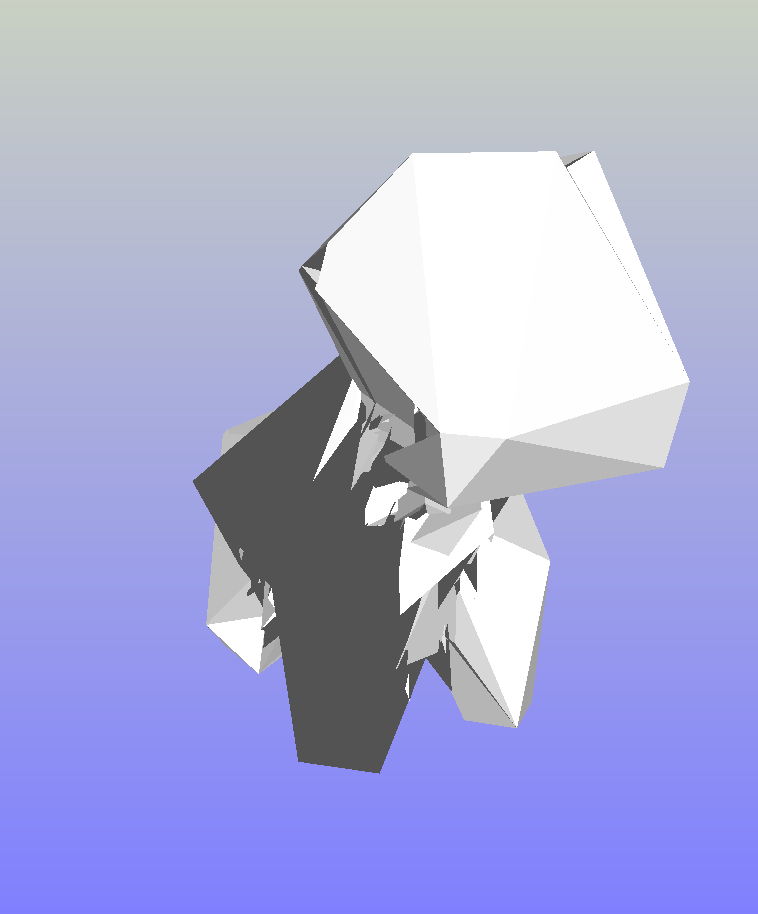
\includegraphics[width=\linewidth]{./figures/spot-raw.png}
                    \caption{Naive, 1000}

                \column[]{.25\textwidth}
                    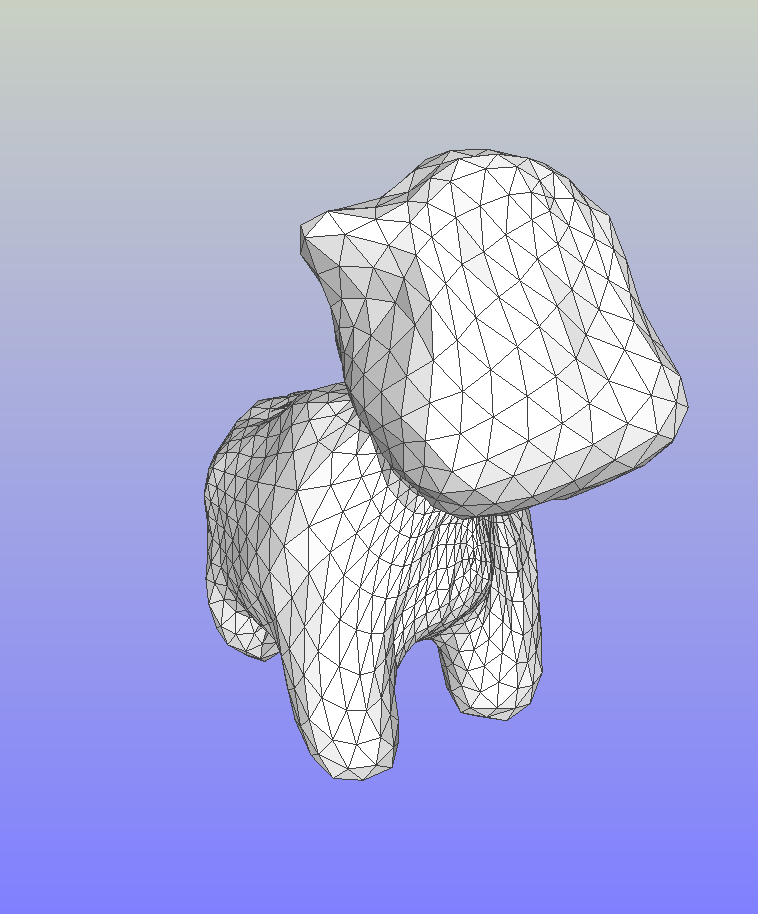
\includegraphics[width=\linewidth]{./figures/spot-reg.png}
                    \caption{Regularaization, 1000}

                \column[]{.25\textwidth}
                    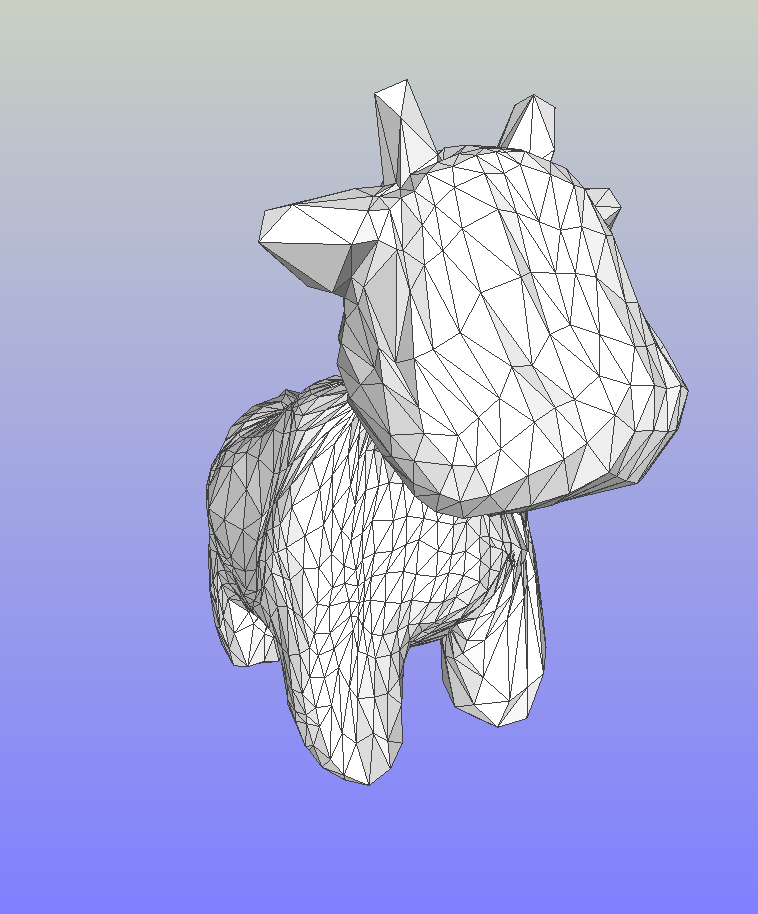
\includegraphics[width=\linewidth]{./figures/spot-new.png}
                    \caption{Gradient filtering, 100}
            \end{columns}
        \end{figure}

\end{frame}

\end{document}